\documentclass[aspectratio=169]{beamer}

% Shared preamble for Claude Code slide decks
% Usage: % Shared preamble for Claude Code slide decks
% Usage: % Shared preamble for Claude Code slide decks
% Usage: \input{preamble} after \documentclass[aspectratio=169]{beamer}

\usetheme{default}
\usecolortheme{dove}

\setbeamertemplate{navigation symbols}{}
\setbeamertemplate{footline}{%
  \hfill{\large\insertframenumber\,/\,\inserttotalframenumber}\hspace{0.8em}\vspace{0.5em}%
}

\definecolor{popblue}{RGB}{52, 101, 164}
\definecolor{sampred}{RGB}{204, 0, 0}
\definecolor{paramgreen}{RGB}{0, 140, 70}
\definecolor{lightbg}{RGB}{245, 245, 250}
\definecolor{warnred}{RGB}{180, 40, 40}
\definecolor{orange1}{RGB}{220, 120, 0}
\definecolor{violet1}{RGB}{120, 50, 160}

\setbeamercolor{frametitle}{fg=popblue}
\setbeamercolor{title}{fg=popblue}
\setbeamercolor{block title}{fg=white,bg=popblue}
\setbeamercolor{block body}{bg=lightbg}
\setbeamercolor{block title alerted}{fg=white,bg=warnred}
\setbeamercolor{block body alerted}{bg=lightbg}
\setbeamercolor{block title example}{fg=white,bg=paramgreen}
\setbeamercolor{block body example}{bg=lightbg}

\usepackage{listings}
\usepackage[T1]{fontenc}
\usepackage{hyperref}
\usepackage{tikz}
\usepackage{booktabs}
\usetikzlibrary{shapes, arrows.meta, positioning, calc}

\lstset{
  basicstyle=\ttfamily\scriptsize,
  keywordstyle=\color{popblue}\bfseries,
  stringstyle=\color{paramgreen},
  commentstyle=\color{gray},
  breaklines=true,
  frame=single,
  backgroundcolor=\color{lightbg},
  rulecolor=\color{popblue!30},
  showstringspaces=false,
  columns=fullflexible,
}
 after \documentclass[aspectratio=169]{beamer}

\usetheme{default}
\usecolortheme{dove}

\setbeamertemplate{navigation symbols}{}
\setbeamertemplate{footline}{%
  \hfill{\large\insertframenumber\,/\,\inserttotalframenumber}\hspace{0.8em}\vspace{0.5em}%
}

\definecolor{popblue}{RGB}{52, 101, 164}
\definecolor{sampred}{RGB}{204, 0, 0}
\definecolor{paramgreen}{RGB}{0, 140, 70}
\definecolor{lightbg}{RGB}{245, 245, 250}
\definecolor{warnred}{RGB}{180, 40, 40}
\definecolor{orange1}{RGB}{220, 120, 0}
\definecolor{violet1}{RGB}{120, 50, 160}

\setbeamercolor{frametitle}{fg=popblue}
\setbeamercolor{title}{fg=popblue}
\setbeamercolor{block title}{fg=white,bg=popblue}
\setbeamercolor{block body}{bg=lightbg}
\setbeamercolor{block title alerted}{fg=white,bg=warnred}
\setbeamercolor{block body alerted}{bg=lightbg}
\setbeamercolor{block title example}{fg=white,bg=paramgreen}
\setbeamercolor{block body example}{bg=lightbg}

\usepackage{listings}
\usepackage[T1]{fontenc}
\usepackage{hyperref}
\usepackage{tikz}
\usepackage{booktabs}
\usetikzlibrary{shapes, arrows.meta, positioning, calc}

\lstset{
  basicstyle=\ttfamily\scriptsize,
  keywordstyle=\color{popblue}\bfseries,
  stringstyle=\color{paramgreen},
  commentstyle=\color{gray},
  breaklines=true,
  frame=single,
  backgroundcolor=\color{lightbg},
  rulecolor=\color{popblue!30},
  showstringspaces=false,
  columns=fullflexible,
}
 after \documentclass[aspectratio=169]{beamer}

\usetheme{default}
\usecolortheme{dove}

\setbeamertemplate{navigation symbols}{}
\setbeamertemplate{footline}{%
  \hfill{\large\insertframenumber\,/\,\inserttotalframenumber}\hspace{0.8em}\vspace{0.5em}%
}

\definecolor{popblue}{RGB}{52, 101, 164}
\definecolor{sampred}{RGB}{204, 0, 0}
\definecolor{paramgreen}{RGB}{0, 140, 70}
\definecolor{lightbg}{RGB}{245, 245, 250}
\definecolor{warnred}{RGB}{180, 40, 40}
\definecolor{orange1}{RGB}{220, 120, 0}
\definecolor{violet1}{RGB}{120, 50, 160}

\setbeamercolor{frametitle}{fg=popblue}
\setbeamercolor{title}{fg=popblue}
\setbeamercolor{block title}{fg=white,bg=popblue}
\setbeamercolor{block body}{bg=lightbg}
\setbeamercolor{block title alerted}{fg=white,bg=warnred}
\setbeamercolor{block body alerted}{bg=lightbg}
\setbeamercolor{block title example}{fg=white,bg=paramgreen}
\setbeamercolor{block body example}{bg=lightbg}

\usepackage{listings}
\usepackage[T1]{fontenc}
\usepackage{hyperref}
\usepackage{tikz}
\usepackage{booktabs}
\usetikzlibrary{shapes, arrows.meta, positioning, calc}

\lstset{
  basicstyle=\ttfamily\scriptsize,
  keywordstyle=\color{popblue}\bfseries,
  stringstyle=\color{paramgreen},
  commentstyle=\color{gray},
  breaklines=true,
  frame=single,
  backgroundcolor=\color{lightbg},
  rulecolor=\color{popblue!30},
  showstringspaces=false,
  columns=fullflexible,
}


\title{Introduction to Subagents}
\subtitle{Delegation $\cdot$ Custom Agents $\cdot$ Effective Design}
\date{}

\begin{document}

\begin{frame}
\titlepage
\end{frame}

% ──────────────────────────────────────────────
\begin{frame}{What Are Subagents?}
\textbf{Subagents} = separate Claude instances with their own context window, spawned by the main agent to handle specific tasks.

\bigskip
\begin{center}
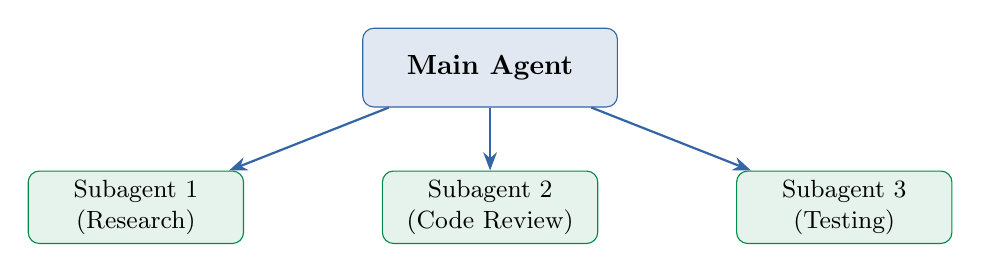
\begin{tikzpicture}[
  node distance=0.8cm and 1.5cm,
  main/.style={rectangle, rounded corners, draw=popblue, fill=popblue!15,
               text width=3cm, minimum height=1cm, align=center, font=\bfseries},
  sub/.style={rectangle, rounded corners, draw=paramgreen, fill=paramgreen!10,
              text width=2.5cm, minimum height=0.8cm, align=center, font=\small},
  arr/.style={-Stealth, thick, popblue}
]
  \node[main] (parent) {Main Agent};
  \node[sub, below left=of parent] (s1) {Subagent 1\\(Research)};
  \node[sub, below=of parent] (s2) {Subagent 2\\(Code Review)};
  \node[sub, below right=of parent] (s3) {Subagent 3\\(Testing)};
  \draw[arr] (parent) -- (s1);
  \draw[arr] (parent) -- (s2);
  \draw[arr] (parent) -- (s3);
\end{tikzpicture}
\end{center}

\begin{itemize}
  \item Each subagent has its own \textbf{separate context window}
  \item Can run \textbf{in parallel} for independent tasks
  \item Results flow back to the parent agent
\end{itemize}
\end{frame}

% ──────────────────────────────────────────────
\begin{frame}{Built-in Subagents}
Claude Code ships with three built-in subagent types:

\bigskip
\begin{columns}[T]
\column{0.33\textwidth}
\begin{block}{General Purpose}
\begin{itemize}
  \item Default agent type
  \item Full tool access
  \item Complex multi-step tasks
\end{itemize}
\end{block}

\column{0.33\textwidth}
\begin{block}{Explore}
\begin{itemize}
  \item Fast codebase search
  \item Find files by pattern
  \item Answer codebase questions
\end{itemize}
\end{block}

\column{0.33\textwidth}
\begin{block}{Plan}
\begin{itemize}
  \item Architecture design
  \item Implementation strategy
  \item Trade-off analysis
\end{itemize}
\end{block}
\end{columns}

\bigskip
You can also create \textbf{custom subagents} tailored to your workflows.
\end{frame}

% ──────────────────────────────────────────────
\begin{frame}[fragile]{Creating a Custom Subagent}
Create a markdown file in \texttt{.claude/agents/}:

\begin{lstlisting}[]
# .claude/agents/security-reviewer.md
---
name: security-reviewer
description: >
  Reviews code changes for security vulnerabilities,
  checks for OWASP top 10 issues, and suggests fixes.
tools:
  - Read
  - Grep
  - Glob
model: opus
isolation: worktree    # isolated repo copy
maxTurns: 20
---

When reviewing code for security issues:
1. Check for injection vulnerabilities (SQL, XSS, command)
2. Verify input validation at system boundaries
3. Check authentication and authorization logic
4. Look for sensitive data exposure
5. Report findings with severity and fix suggestions
\end{lstlisting}
\end{frame}

% ──────────────────────────────────────────────
\begin{frame}{Designing Effective Subagents}
\textbf{\color{popblue}The description is everything} --- it shapes how the parent delegates.

\bigskip
\begin{columns}[T]
\column{0.5\textwidth}
\begin{alertblock}{Bad description}
``Helps with code''
\end{alertblock}
\begin{exampleblock}{Good description}
``Reviews Python code changes for type safety issues, checks mypy compatibility, and suggests type annotations for untyped functions.''
\end{exampleblock}

\column{0.5\textwidth}
\textbf{Design principles:}
\begin{enumerate}
  \item Specific, action-oriented description
  \item Define \textbf{output format}
  \item Instruct: report obstacles,\\don't guess
  \item \textbf{Limit tool access} to what's needed
  \item Consider \textbf{proactive delegation}
\end{enumerate}
\end{columns}
\end{frame}

% ──────────────────────────────────────────────
\begin{frame}{When Subagents Shine vs.\ When They Hurt}
\begin{columns}[T]
\column{0.5\textwidth}
\begin{exampleblock}{Use subagents for}
\begin{itemize}
  \item \textbf{Research} --- explore codebase, gather context in parallel
  \item \textbf{Code reviews} --- isolated analysis with focused tools
  \item \textbf{Custom system prompts} --- specialized behavior per task
  \item \textbf{Parallel independent work}
\end{itemize}
\end{exampleblock}

\column{0.5\textwidth}
\begin{alertblock}{Avoid subagents for}
\begin{itemize}
  \item \textbf{Expert claims} --- ``I'm an expert in X'' doesn't help
  \item \textbf{Sequential pipelines} --- overhead without parallelism benefit
  \item \textbf{Test runners} --- use hooks instead for automatic testing
  \item \textbf{Simple single-step tasks}
\end{itemize}
\end{alertblock}
\end{columns}

\bigskip
\begin{block}{The Decision Rule}
\centering
Use a subagent when the task benefits from \textbf{isolation} (separate context) or \textbf{parallelism} (multiple tasks at once). Otherwise, keep it in the main agent.
\end{block}
\end{frame}

% ──────────────────────────────────────────────
\begin{frame}{Advanced Subagent Features}
\begin{columns}[T]
\column{0.5\textwidth}
\textbf{\color{popblue}Background Execution}
\begin{itemize}
  \item \texttt{background: true} in frontmatter
  \item Or \textbf{Ctrl+B} to background a running task
  \item Auto-denies unapproved permissions
\end{itemize}

\bigskip
\textbf{\color{paramgreen}Worktree Isolation}
\begin{itemize}
  \item \texttt{isolation: "worktree"} in frontmatter
  \item Subagent gets an isolated repo copy
  \item Enables safe parallel development
\end{itemize}

\column{0.5\textwidth}
\textbf{\color{orange1}Persistent Memory}
\begin{itemize}
  \item \texttt{memory} field: \texttt{user}, \texttt{project}, or \texttt{local}
  \item Knowledge accumulates across sessions
\end{itemize}

\bigskip
\textbf{\color{violet1}Invocation Methods}
\begin{itemize}
  \item Natural language (auto-delegation)
  \item \texttt{@"reviewer (agent)"} (explicit)
  \item \texttt{claude --agent reviewer} (session-wide)
\end{itemize}
\end{columns}
\end{frame}

% ──────────────────────────────────────────────
\begin{frame}{Agent Teams (Research Preview)}
\textbf{Agent Teams} = multiple Claude sessions coordinating across separate processes.

\bigskip
\begin{center}
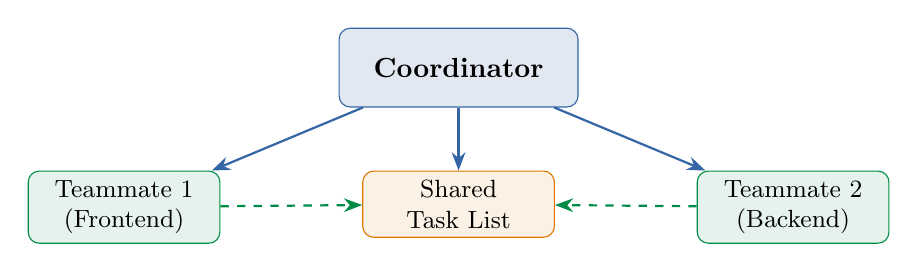
\begin{tikzpicture}[
  node distance=0.8cm and 1.5cm,
  main/.style={rectangle, rounded corners, draw=popblue, fill=popblue!15,
               text width=2.8cm, minimum height=1cm, align=center, font=\bfseries},
  sub/.style={rectangle, rounded corners, draw=paramgreen, fill=paramgreen!10,
              text width=2.2cm, minimum height=0.8cm, align=center, font=\small},
  shared/.style={rectangle, rounded corners, draw=orange1, fill=orange1!10,
                text width=2.2cm, minimum height=0.8cm, align=center, font=\small},
  arr/.style={-Stealth, thick, popblue}
]
  \node[main] (coord) {Coordinator};
  \node[sub, below left=of coord] (t1) {Teammate 1\\(Frontend)};
  \node[shared, below=of coord] (tasks) {Shared\\Task List};
  \node[sub, below right=of coord] (t2) {Teammate 2\\(Backend)};
  \draw[arr] (coord) -- (t1);
  \draw[arr] (coord) -- (tasks);
  \draw[arr] (coord) -- (t2);
  \draw[arr, dashed, paramgreen] (t1) -- (tasks);
  \draw[arr, dashed, paramgreen] (t2) -- (tasks);
\end{tikzpicture}
\end{center}

\begin{block}{Key difference from subagents}
Subagents work \emph{within} a single session. Agent teams coordinate \emph{across} separate sessions with shared task lists and mailbox systems.
\end{block}
\end{frame}

% ──────────────────────────────────────────────
\begin{frame}{Summary}
\begin{block}{Key Takeaways}
\begin{itemize}
  \item Subagents = separate Claude instances with their own context
  \item Built-in: General Purpose, Explore, Plan
  \item Custom subagents via \texttt{.claude/agents/*.md} with frontmatter
  \item Description quality determines delegation quality
  \item Advanced: background execution, worktree isolation, persistent memory
  \item Agent Teams = multi-session coordination (research preview)
  \item Best for: research, reviews, parallel work
\end{itemize}
\end{block}

\vfill
\centering
\Large\color{popblue} Questions?
\end{frame}

\end{document}
